\chapter{Camera Pose Verification}

In the chapter, datasets, their transformations, and experiments performed upon them with
the introduced methods' implementations are all presented. We use the generalized InLoc
pipeline with a modified pose verification step. The synthesized image leveraged for
pixel-wise computation of similarity with the given query image is swapped with views
generated by renderers presented in the preceding chapter, depicting the scene's point
cloud from estimated query positions. Apart from how the synthesized image is generated,
the rest of the verification process is then performed according to the original article,
using namely RootSIFT descriptors.\\

While discussing concrete details of datasets' definitions and algorithms' inputs, more
technical aspects are taken into account---among them, of utmost importance are
conventions used by coordinate systems in which points of explicit scene representations
are expressed/expected to be and by matrices related to cameras taking database images.
These pose a crucial difference between what a dataset provides, or localization pipeline
expects and must be addressed by implementation to obtain valid localization results.

\begin{figure}
    \centering
    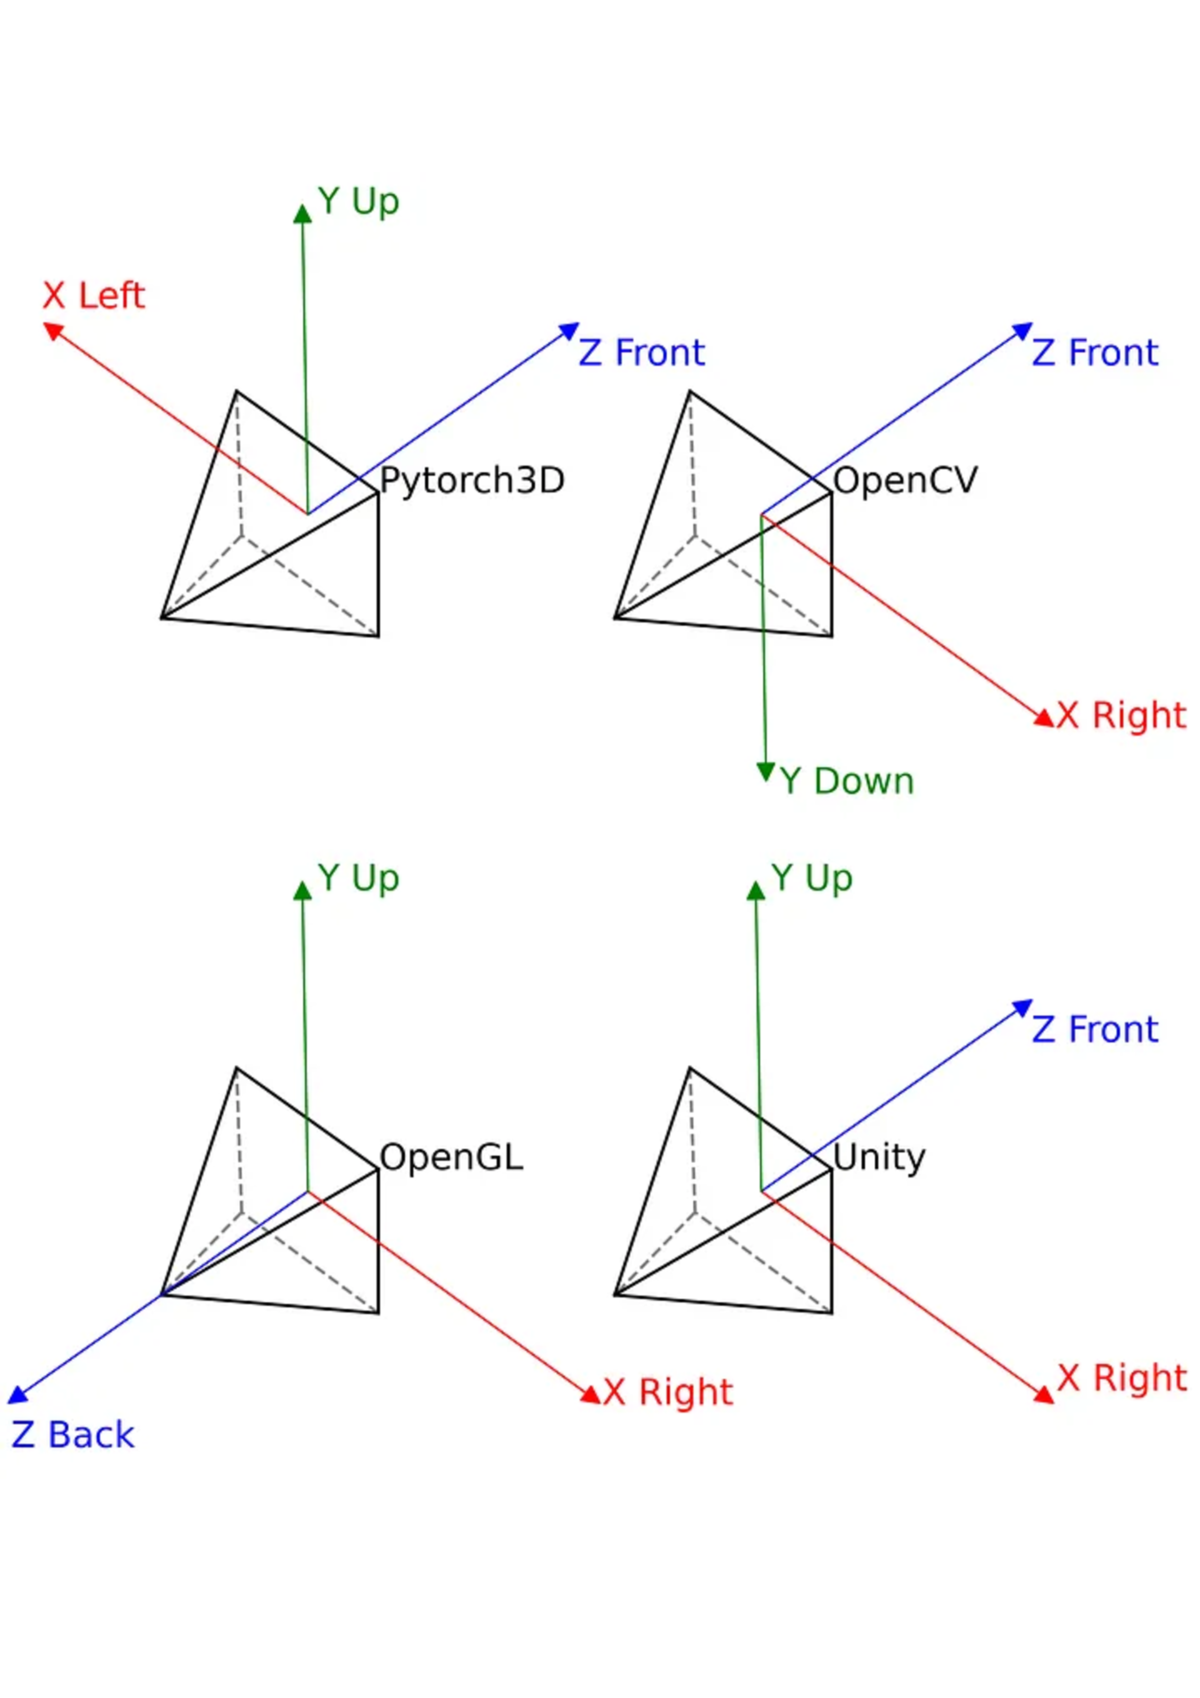
\includegraphics[width=.7\textwidth]{../graphics/cs_conventions.png}
    \caption[Examples of various camera\,/\,coordinate frame conventions]{
    Examples of various camera\,/\,coordinate frame conventions used by
    common programmatic tools in fields dealing with computer graphics.
    Taken from~\url{https://medium.com/check-visit-computer-vision/converting-camera-poses-from-opencv-to-opengl-can-be-easy-27ff6c413bdb}.}\label{fig:cs_conventions}
\end{figure}

Coordinate system conventions address the decision of assigning positive directions,
labels, and meanings in the human sense (up, right, forward) to the orthogonal frame of a
3D space, because without that an oriented triplet representing a point is meaningless.
These conventions can be arbitrary depending on whether they come from computer vision,
rendering, or another field. Examples of such conventions, linked to standard computer
graphics libraries/tools that use/expect them, can be found in~\cref{fig:cs_conventions}.
In this thesis, computer vision and rendering conventions are used. In the
figure~\cref{fig:cs_conventions}, these are found alongside OpenCV and OpenGL labels,
respectively. Even though both are right-handed, they understand x, y, and z point
components differently.  In rendering, the positive x-axis points to the right, the
positive y-axis up, and the positive z-axis towards a viewer looking at the coordinate
system frame. In computer vision, the positive x-axis points to the right, the positive
y-axis to the bottom, and the z-axis away from the same viewer as before. Transformation
matrices operating over both notations are thus related by inverting the y and z axes
columns. As an example, since a camera in rendering is typically placed along z-xis,
failing to take this relation into account when displaying a 3D model defined in computer
vision notation in a visualization tool that uses rendering notation results in rendering
half-space \uv{away} from the model. For instance, in the case of other notations used by
a produced model, a rendered view can be somewhat unexpectedly rotated.

Matrix conventions in the context of the thesis are related to terms coming from the
graphics pipeline---\emph{world space} and \emph{view space}. In the case of datasets
described below, world space is a space of the whole scene representation with the origin
and orientation of the coordinate frame chosen arbitrarily in relation to the scene.  The
randomness in the coordinate frame placement is especially true in the case of
SfM-generated scene models, where the algorithm decides these parameters.  When preparing
a model manually, e.g., in the game industry, the frame is typically artificially placed
meaningfully concerning the model produced, e.g., along the outer edges of a cube model.
View space is a space of a camera looking at a portion of the scene---origin is the center
of the camera with the coordinate frame oriented in a specific way alongside the optical
axis of the camera depending on the exact graphics pipeline/tool used.
Visualisation~\cref{fig:cs_conventions} can be used here as well---the square pyramids
depict view frustums of virtual cameras, with the z-axes being their optical axes.

Provided both spaces are same-handed, the matrix inverse relates transformations between
them. In homogeneous coordinates, both transformations are represented by $4\times4$
matrices, and the implementation must correctly distinguish between the actual meaning of
these 16~real numbers, including how the matrix is stored on the disk. We refer to them as
the \emph{view matrix} transforming from world to view space and \emph{camera pose}
representing the opposite, inverse transformation.
